\section{Works Done}
\label{sec:worksDone}
\subsection{Food Tank Construction}
Food tank is the unit to store food and feed cat whenever required. The tank design was done in the first week which is implemented this week. Figure \ref{fig:mamaKabi} shows the look of tank from different viewpoints. A motor will be mounted to the bottom part of the tank so that trigger mechanism can easily control the flow of food. Since there is no cat food present at the moment, the test stage will be handled next week.

\begin{figure}
    \centering
    \begin{subfigure}[b]{0.49\textwidth}
        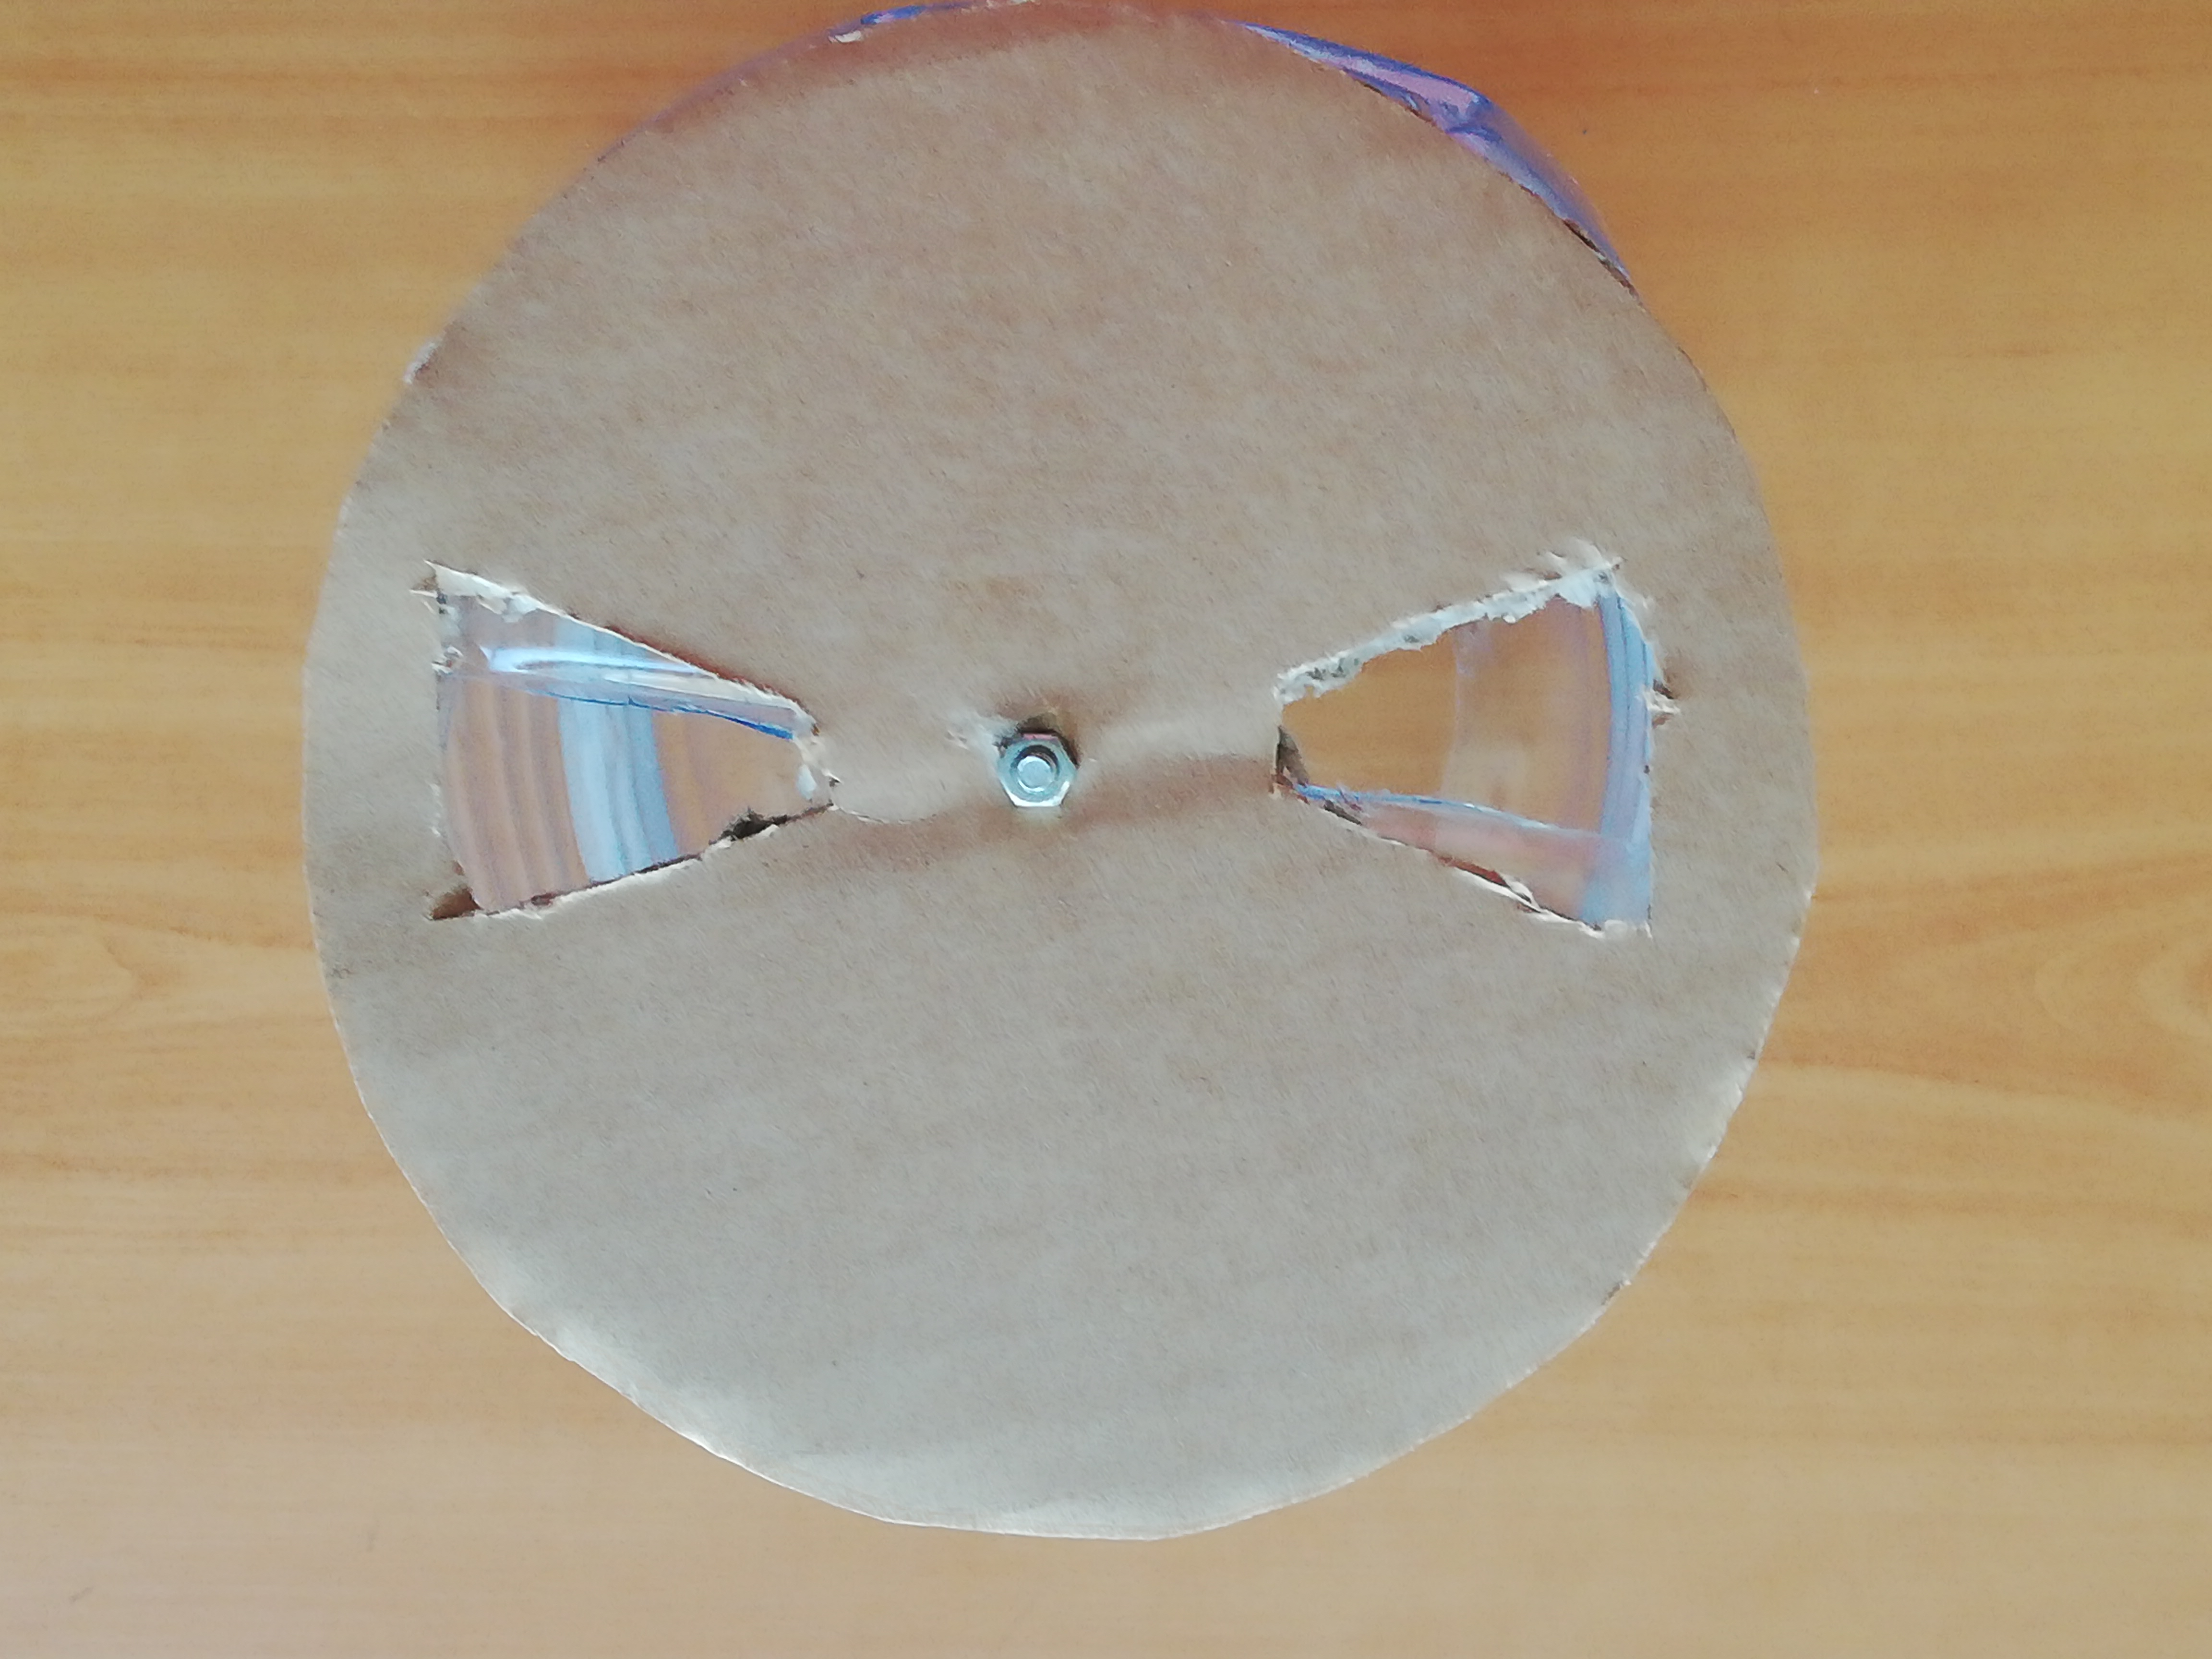
\includegraphics[width=\textwidth]{img/tank1.jpg}
        \caption{Top View}
        \label{fig:mamaKabi1}
    \end{subfigure}
    \begin{subfigure}[b]{0.49\textwidth}
        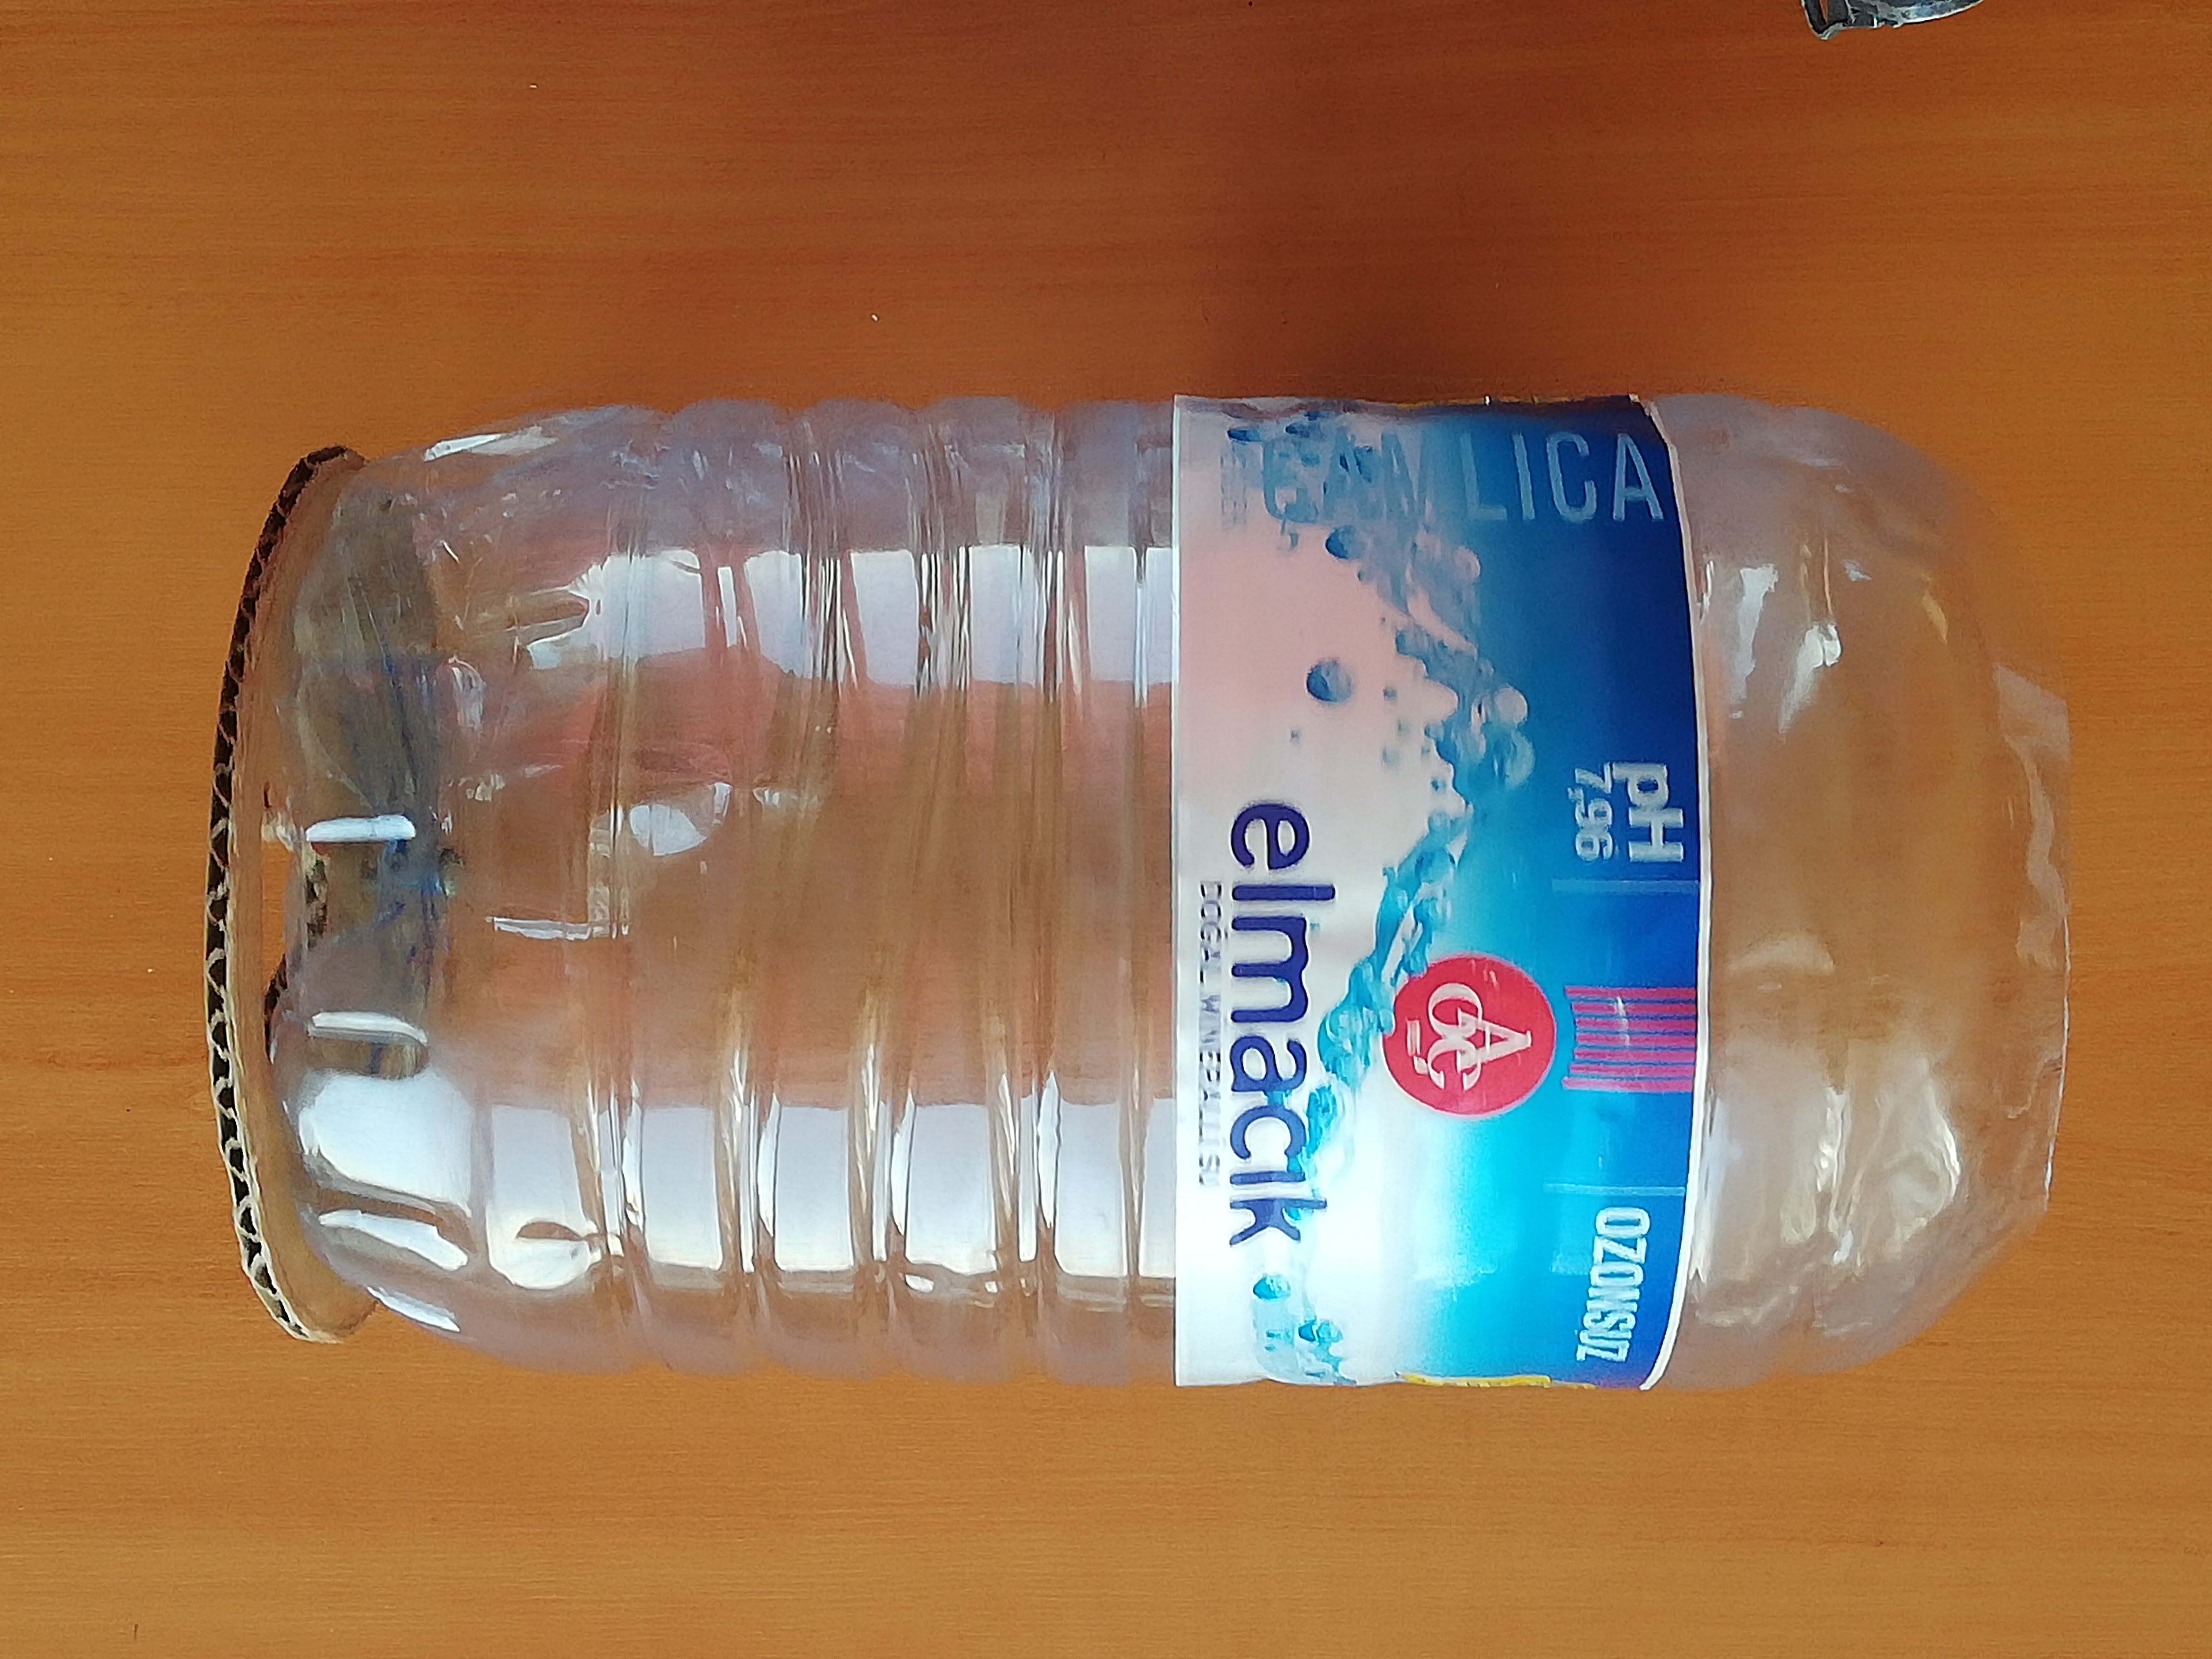
\includegraphics[width=\textwidth]{img/tank2.jpg}
        \caption{Lateral View}
        \label{fig:mamaKabi2}
    \end{subfigure}
    \begin{subfigure}[b]{0.49\textwidth}
        \includegraphics[width=\textwidth]{img/tank3.jpg}
        \caption{Bottom View}
        \label{fig:mamaKabi3}
    \end{subfigure}
     \begin{subfigure}[b]{0.49\textwidth}
        \includegraphics[width=\textwidth]{img/tank4.jpg}
        \caption{Angled View}
        \label{fig:mamaKabi3}
    \end{subfigure}
    \caption{Food Tank}
    \label{fig:mamaKabi}
\end{figure}

\subsection{Environment Setup}
Each team member installed required software and environment onto their personal computers. Moreover, registrations to cloud computing platforms are done with student packs got from GitHub Student Pack utility\cite{cite:github_studentPack}.